\documentclass{article} % For LaTeX2e
\usepackage{iclr2027_conference,times}

% Optional math commands from https://github.com/goodfeli/dlbook_notation.
\input{math_commands.tex}

\usepackage{hyperref}
\usepackage{url}
\usepackage{booktabs}
\usepackage{graphicx}
\usepackage{amsmath}
\usepackage{amssymb}
\usepackage{xcolor}
\usepackage{multirow}

\newcommand{\fix}{\marginpar{FIX}}
\newcommand{\new}{\marginpar{NEW}}

\title{Never Formed or Later Lost? Measuring Correct-Answer Output-Space Dynamics in Large Language Models}

% Authors hidden for anonymous submission
\author{Anonymous Author(s) \\
Affiliation \\
Address \\
\texttt{email}
}

%\iclrfinalcopy % Uncomment for camera-ready version, but NOT for submission.
\begin{document}

\maketitle

\begin{abstract}
A wrong answer can arise from at least two distinct output-space trajectories: the gold answer may never become a competitive candidate, or it may become competitive at an intermediate layer and later lose that status. Distinguishing these cases requires more than showing that the gold token once exceeded a single wrong token. We introduce \emph{Information Dynamics}, an operational framework that traces the gold answer's log-probability, full-vocabulary rank, and competitor-relative margin across Transformer layers. Across six open-weight instruction-tuned models (4B--14B parameters) and seven tasks, we find that the common ``ever crossing'' shortcut is non-diagnostic: it occurs in 92.2\% of errors, while random and strength-matched competitor nulls yield still higher rates (98.8\% and 98.7\%). Under a stricter vocabulary-wide criterion, preservation failures form a small, task-dependent subset of errors (10.0\% on the Qwen3-8B seven-task error set; 95\% CI [8.4\%, 11.4\%]), whereas most errors never exhibit an output-competitive gold signal under the evaluated decoder. Early trajectory shape also contains predictive information about later decay: an endpoint-conditioned retrospective classifier reaches AUC $0.75\pm0.02$, while an endpoint-free gold-token variant reaches 0.66. Finally, final-rank-matched restoration experiments provide evidence that errors with a strong intermediate gold state are more repairable than errors without one. We release \texttt{InfoDyn-Bench} to support further work on layer-wise error diagnosis. Our claims concern output-space decodability, not a general definition of what a model ``knows.''
\end{abstract}

\section{Introduction}

When a language model produces a wrong answer, the final output does not reveal how that failure developed \citep{ji2023survey, huang2023survey}. At the position where the answer begins, the gold token may never become competitive in the decoded vocabulary distribution, or it may become competitive at an intermediate layer and later lose that status. These cases are observationally identical at the output but are different operational diagnoses. The first indicates that the evaluated readout never exposes an output-ready gold candidate; the second identifies a candidate signal that later computation does not preserve. We deliberately avoid equating either diagnosis with an unrestricted claim about whether the model ``knows'' the answer.

Making this distinction is harder than inspecting a pair of logits. Prior layer-wise analyses often ask whether the gold token ever outranks the final wrong token. We show that this event is almost ubiquitous even under null competitors: the observed crossing rate is 92.2\%, while random and final-strength-matched competitor nulls yield 98.8\% and 98.7\%. Beating one token at one layer therefore does not establish vocabulary-wide competitiveness.

We introduce \emph{Information Dynamics}, which tracks the gold token's layer-wise log-probability, full-vocabulary rank, and margin relative to a fixed final competitor. The primary taxonomy is defined at the \emph{answer-onset token} in the model's actual generation context. A signal is operationally competitive only if it is both near the top of the vocabulary and ahead of the eventual competitor under the specified decoder. An incorrect example is a formation failure when this event is never observed and a preservation failure when the event is observed at an intermediate layer but not at the final layer. This is a definition of decoded output readiness, not of all information that may be nonlinearly encoded elsewhere in the network.

Across six models and seven tasks, three conclusions are consistent. First, pairwise sign flips are too weak to support claims of prior signal formation. Second, under the strict vocabulary-wide criterion, preservation failures are a minority: 10.0\% of 1{,}494 Qwen3-8B errors, with strong task dependence and no detected cases on GSM8K under this criterion. Third, the distinction has behavioral relevance. In final-rank-matched pairs, restoring the intermediate peak state recovers 12.3\% of preservation failures versus 1.8\% of formation failures, although the paired test is only marginal ($p=0.070$) and we treat this result as directional rather than definitive. Direction-targeted patches provide additional evidence, but because they use the gold direction, we interpret them as oracle mechanism probes rather than deployable repair methods.

We also study prediction as a secondary, retrospective analysis. A first-half trajectory classifier reaches AUC $0.75\pm0.02$ when its margin is defined against the endpoint-selected competitor. Because the competitor identity comes from the final layer, this number is endpoint-conditioned rather than a purely online forecast. An endpoint-free variant using only the gold token's rank and log-probability reaches AUC 0.66. A separate gold-free candidate-dynamics predictor is evaluated only within a pool of known errors and therefore does not by itself solve end-to-end error detection.

Our contributions are:
\begin{enumerate}
    \item \textbf{A measurement critique.} We demonstrate with random and strength-matched nulls that ``gold ever beats the final wrong token'' is a non-diagnostic criterion.
    \item \textbf{An operational error taxonomy.} We define formation and preservation failures using vocabulary-wide competitiveness at the actual answer-onset position, and report a strict, task-dependent preservation regime while keeping alternative multi-token criteria separate.
    \item \textbf{Behavioral validation.} Final-rank-matched restoration and direction-targeted interventions show that examples with a competitive intermediate gold state are more amenable to oracle repair, while also exposing the limits of gold-conditioned interventions.
    \item \textbf{Trajectory analyses and resource.} We quantify retrospective decay prediction, cross-task and cross-model transfer, and release \texttt{InfoDyn-Bench} with explicit metric definitions and analysis splits.
\end{enumerate}

\section{Related Work}

\subsection{Decoding Intermediate Representations}
Logit lens \citep{nostalgebraist2020logitlens} and tuned lens \citep{belrose2023tunedlens} decode intermediate hidden states back into the vocabulary space. Probing studies ask whether linguistic or factual information is decodable at specific layers using diagnostic classifiers \citep{alain2016understanding, tenney2019bert, hewitt2019structural, belinkov2022probing}. Short-circuiting and early exit approaches study early prediction readiness \citep{schuster2022confident, din2023jump}. These works ask whether a signal is \emph{present} at a given layer. We instead study how a correct-answer signal \emph{evolves dynamically across layers} and systematically quantify readout and selection biases.

\subsection{Knowledge and Factual Recall}
Work on factual knowledge localization, knowledge neurons, and model editing asks where factual associations are stored in feed-forward layers \citep{geva2021transformer, dai2022knowledge, meng2022rome, meng2023memit, geva2023dissecting}. Known-versus-unknown detection and latent knowledge discovery investigate whether internal representations track model correctness \citep{kadavath2022language, burns2022discovering, azaria2023internal, yin2023do, li2024inference}. We do not aim to edit or locate static facts; instead, we track how the correct-answer signal dynamically rises or decays along the network's depth dimension.

\subsection{Hallucination and Error Prediction}
Uncertainty estimation, hidden-state failure prediction, and hallucination detection analyze intermediate representations to identify potential errors \citep{schuster2022confident, kuhn2023semantic, azaria2023internal, manakul2023selfcheckgpt}. Most directly related to our work, \citet{jiang2024hallucination} study layer-wise inference dynamics of correct versus hallucinated outputs using residual-stream decoding and report that dynamic probability curves can predict hallucination. \citet{kim2025uncertainty} extend this to uncertainty-aware layer-wise analysis across multiple models and datasets. Our work differs in three concrete ways: (i)~we demonstrate that naive pairwise logit crossings are explained by an endpoint-conditioned selection bias, establishing a calibration step that prior layer-wise analyses do not include; (ii)~we distinguish formation failures from preservation failures as an operational taxonomy rather than treating all layer-wise dynamics as a single phenomenon; and (iii)~we evaluate whether early-trajectory features carry predictive information \emph{beyond} simple temporal extrapolation (AR baselines, final-layer confidence), whereas prior work predicts error versus correct output categories without ablating temporal autocorrelation.

\subsection{Mechanistic Interpretability and Causal Intervention}
Transformer circuit analysis, direct logit attribution, and activation patching decompose network computations into functional components \citep{elhage2021mathematical, olsson2022incontext, wang2022interpretability, nanda2023progress}. Representation engineering and activation steering modify hidden states to alter output behavior \citep{turner2023activation, rimsky2023steering, zou2023representation}. We perform component-level attribution on information trajectories to isolate the late-layer components associated with correct-signal decay, complementing rather than relying on a particular steering method.

Our work combines null-calibrated intermediate readouts with an explicit formation-versus-preservation taxonomy and tests trajectory prediction against temporal-extrapolation baselines.

\section{Problem Definition}
\label{sec:def}

We fix notation here so that every symbol is defined once.

\subsection{Setup}
Let $x$ be a question, $y^\star$ the gold-answer token, and $\hat{y}$ the token the model actually generates. Let $L$ be the number of layers. At layer $\ell$ ($1 \le \ell \le L$), let $h_\ell(x) \in \mathbb{R}^d$ be the hidden representation at the target position, where $d$ is the hidden dimension. Let $W_U \in \mathbb{R}^{d \times |V|}$ denote the unembedding matrix, where $|V|$ is the vocabulary size, and let $w_y \in \mathbb{R}^d$ be the unembedding vector corresponding to token $y$. A lens $g_\ell$ maps the representation to a logit vector, which we turn into a distribution over the vocabulary by a softmax:
\begin{equation}
p_\ell(y \mid x) = \operatorname{softmax}(g_\ell(h_\ell(x)))_y .
\end{equation}
We use two lenses. The raw logit lens \citep{nostalgebraist2020logitlens} sets $g_\ell$ to the final language-model head, applying the final layer norm and unembedding matrix $W_U$. The tuned lens \citep{belrose2023tunedlens} adds a per-layer affine map that is trained so that the decoded logits approximate the final-layer logits.

We define the \emph{gold rank} $r_\ell(y^\star)$ as the number of tokens whose probability at layer $\ell$ strictly exceeds that of the gold answer. With this zero-based convention, $r_\ell(y^\star) = 0$ means that the gold answer is top-1:
\begin{equation}
r_\ell(y^\star) = \sum_{y \neq y^\star} \mathbb{1}\big[ p_\ell(y) > p_\ell(y^\star) \big] .
\end{equation}
All reported ranks use this zero-based convention. The experiments were run with the stored cutoff $r_\ell\leq 5$, which admits at most five tokens above the gold token (i.e., rank at most six in one-based terminology). For transparency, we call this the \emph{$k=5$ competitiveness cutoff} rather than the conventional ``top-5'' in the revised text. The neighboring-threshold analysis in Appendix~\ref{app:thresholds} shows how the conclusions vary with the cutoff.

\subsection{Two Competitive Margins}
We use two related margins in different analyses. The first compares the gold answer with the generated answer $\hat{y}$:
\begin{equation}
\mathrm{CIS}^{\mathrm{gen}}_\ell = \log p_\ell(y^\star) - \log p_\ell(\hat{y}), \qquad \hat{y} \neq y^\star .
\end{equation}
We use this margin for error examples and for the endpoint-bias analysis. The second compares the gold answer with the strongest competing token $y^-$, defined as the most probable token other than the gold answer at the final layer:
\begin{equation}
y^- = \arg\max_{y \neq y^\star} p_L(y), \qquad
\mathrm{CIS}^{\mathrm{comp}}_\ell = \log p_\ell(y^\star) - \log p_\ell(y^-) .
\end{equation}
We fix $y^-$ at the final layer and track it across depths so that the pairwise margin always refers to the same token. This makes the trajectory comparable across layers, but it also makes the margin \emph{endpoint-conditioned}: the reference token is chosen using the final layer. We therefore do not use this margin as evidence of vocabulary-wide competitiveness by itself. The strict taxonomy requires both $r_\ell\leq k$ and $\mathrm{CIS}^{\mathrm{comp}}_\ell>0$, while the prediction section separately reports a gold-only variant that does not reference $y^-$. A per-layer strongest competitor would avoid endpoint selection but would change identity at every depth and would make a positive margin equivalent to the gold token being top-1. Appendix~\ref{app:metric} states which object each analysis uses.

\subsection{Information Trajectory}
The information trajectory of an example is the per-layer collection of the gold log-probability, the gold rank, and the competitive margin:
\begin{equation}
\mathcal{T}(x) = \big\{ \log p_\ell(y^\star),\; r_\ell(y^\star),\; \mathrm{CIS}^{\mathrm{comp}}_\ell \big\}_{\ell=1}^{L} .
\end{equation}
From this trajectory we derive three quantities. The \emph{peak rank} is the smallest rank over all layers except the final one:
\begin{equation}
r_{\mathrm{peak}} = \min_{1 \le \ell < L} r_\ell(y^\star) .
\end{equation}
The \emph{peak-to-final decay} $D$ is the drop from the largest intermediate margin to the final margin:
\begin{equation}
D = \max_{1 \le \ell < L} \mathrm{CIS}^{\mathrm{comp}}_\ell \;-\; \mathrm{CIS}^{\mathrm{comp}}_L .
\end{equation}
Our primary strict label is the \emph{answer-onset competitive-decay} label. It marks an incorrect example whose first gold answer token satisfies the joint competitiveness criterion at an intermediate layer but loses to the fixed competitor at the final layer:
\begin{equation}
C(x) = \mathbb{1}\Big[ \exists\, \ell < L : r_\ell(y^\star) \le k \;\land\; \mathrm{CIS}^{\mathrm{comp}}_\ell > 0 \Big] \cdot \mathbb{1}\Big[ \mathrm{CIS}^{\mathrm{comp}}_L < 0 \Big] .
\end{equation}
We use the stored cutoff $k=5$ and report sensitivity over $k \in \{1,5,10,50\}$ (Section~\ref{sec:taskdecay}). Because $y^-$ is endpoint-selected, we call Eq.~8 a \emph{strict retrospective taxonomy}; it is not an online or endpoint-free diagnostic.

The cutoff marks a pronounced transition in output-space decodability. At the first layer where the gold token satisfies $r_\ell\leq k$, its log-probability increases by about $8$ log units, from a median near $-11$ to a median near $-2.7$ at $k=5$; the increase is positive in 97\% of samples and remains large for $k\in\{1,5,10\}$. This observation motivates a small-rank competitiveness band, but it does not make any single cutoff uniquely correct. We consequently report threshold sensitivity and interpret the taxonomy as operational.

\paragraph{Scope and multi-token answers.}
The primary taxonomy tracks the first answer token $y^\star_1$ at the actual answer-onset position. This choice keeps the hidden state on the model's realized generation path and makes the measurement comparable across single- and multi-token answers. It does not establish that an entire multi-token answer sequence formed.

For sensitivity analysis only, we also compute a permissive minimum-over-tokens statistic:
\begin{equation}
r^{\mathrm{multi}}_\ell = \min_{1 \le i \le m} r_\ell(y^\star_i) .
\end{equation}
This statistic asks whether \emph{any} constituent token is competitive and is therefore length-biased; it is not our primary failure label.

We additionally perform a \emph{counterfactual teacher-forced sequence-decodability analysis}. We append the gold answer, condition each answer position on the gold prefix, and aggregate token-wise ranks with three rules: \textbf{ALL} (all tokens satisfy the cutoff at the same layer), \textbf{MEAN} (mean rank satisfies the cutoff), and \textbf{JOINT} (intermediate sequence log-likelihood exceeds final sequence log-likelihood). These hidden states are not states visited during the original wrong generation. Moreover, ALL and MEAN measure intermediate formation under gold-prefix conditioning; they do not by themselves require a subsequent final-layer loss. We therefore report them as boundary analyses rather than as preservation-failure rates. On 1{,}494 Qwen3-8B errors, the ALL, MEAN, and JOINT rates are 13.2\%, 25.0\%, and 87.8\%, respectively. The large disagreement demonstrates why these quantities must not be conflated with Eq.~8.

\subsection{Error Taxonomy}
We define four operational categories under the answer-onset measurement. A \emph{formation failure} is an incorrect example whose first gold token never meets the strict joint criterion at an intermediate layer. A \emph{preservation failure} is an incorrect example for which Eq.~8 is positive. A \emph{successful preservation} is a correct example whose first-token signal forms and remains competitive. The remaining category, \emph{unresolved}, covers cases for which answer-onset tracking does not adequately characterize the error, particularly multi-step reasoning and long sequence answers. These labels describe the evaluated output-space readout and should not be interpreted as an exhaustive taxonomy of internal computation.

\section{Experimental Setup}

\subsection{Models and Tasks}
We evaluate three open-weight instruction-tuned model families spanning several scales: Qwen3-14B, Qwen3-8B, Qwen3-4B, and Qwen2.5-7B for scale variation within Qwen, plus Llama-3.1-8B \citep{dubey2024llama} and Mistral-7B-Instruct-v0.3 \citep{jiang2023mistral}. We use seven tasks: TriviaQA \citep{joshi2017triviaqa} for fact QA, HotpotQA \citep{yang2018hotpotqa} for multi-hop QA, GSM8K \citep{cobbe2021gsm8k} for math reasoning, CommonsenseQA for commonsense reasoning, ARC-Challenge for science reasoning, QuALITY for long-context comprehension, and MMLU (four subjects) for world knowledge.

% AUTHOR ACTION REQUIRED BEFORE SUBMISSION:
% Add a compact reproducibility table specifying, for every model/task:
% evaluated sample count, accuracy/error count, prompt template, decoding rule,
% maximum generation length, chain-of-thought policy, MMLU subjects, and
% context truncation. These facts are not stated in the source manuscript and
% must not be guessed during editing.

\subsection{Answer Extraction}
We judge correctness by normalized substring matching after lower-casing. For numeric answers, we strip commas and percent signs and compare numerically with a small tolerance. For TriviaQA, a match against any supplied alias counts as correct. This automatic evaluator is a practical choice but can misclassify negated, embedded, or unusually formatted answers; we list it as a limitation rather than treating it as a semantic judge.

\subsection{Lens Construction}
The raw logit lens applies the final language-model head directly. For the tuned lens \citep{belrose2023tunedlens}, we fit a per-layer affine translator whose decoded logits approximate the model's final-layer logits (Adam, learning rate $10^{-3}$, 500 epochs, independently by layer on held-out prompts). The translator never observes gold answers or correctness labels, so it does not leak downstream labels. It is nevertheless \emph{final-prediction aligned}, not an unbiased view of all intermediate information: on an error, its target is the model's final wrong distribution. We therefore use it as one decoder among several and report raw-lens and parameter-free cosine-probe robustness in Appendix~\ref{app:probe}.

\subsection{Statistical Testing}
We report bootstrap 95\% confidence intervals for key proportions where sample size permits and show per-model or per-task results alongside aggregates. For matched interventions, we report both paired bootstrap intervals and the exact McNemar test; we do not call a result statistically decisive when the exact test does not reach 0.05.

\section{Results}

\subsection{Pairwise Sign Flips Fail to Establish Intermediate Signal Competitiveness}

\paragraph{Testing the shortcut against null baselines.}
We first evaluate the common shortcut of checking whether the gold answer's intermediate probability ever exceeds that of the final incorrect prediction. Across error examples, we observe that the gold token's log-probability surpasses the final competitor at some intermediate layer in 92.2\% of cases. To assess whether this is meaningful, we construct two null baselines. First, a \emph{random-competitor null}: for each error, we replace the true final competitor with the generated token from a different, randomly selected error example. Second, a \emph{rank-matched null}: we select replacement competitors whose final-layer log-probability is within $\pm 1$ logit of the true competitor, controlling for competitor strength. Under both nulls the crossing rate is even higher: 98.8\% $\pm$ 0.4\% for random competitors and 98.7\% $\pm$ 0.4\% for rank-matched competitors (200 permutations, 95\% CI [98.0\%, 99.6\%]). The fact that even strength-matched competitors produce higher crossing rates than the observed rate (92.2\%) shows that the "ever crossing" statistic is simply too weak a criterion: almost any token will be crossed by gold at some layer, regardless of competitor strength or whether the gold signal was ever truly competitive. Pairwise logit crossings therefore offer no empirical evidence that a gold signal was ever meaningfully formed.

\paragraph{Why shortcut analysis misleads.}
Pairwise comparison fails because beating a single wrong token does not imply a high vocabulary rank. The raw and tuned lenses also differ substantially in absolute scale: the raw lens gives a median intermediate peak margin of 4.53, versus 2.24 under the final-prediction-aligned translator on Qwen3-8B (Figure~\ref{fig:bias}, right). We interpret this as decoder sensitivity, not proof that either decoder uniquely recovers the ``true'' intermediate probability. The robust conclusion is therefore based on vocabulary-wide competitiveness and sensitivity across readouts, rather than on the magnitude of a raw pairwise margin.

\begin{figure}[t]
\centering

\includegraphics[width=0.85\textwidth]{figures/fig2_measurement_bias.pdf}
\caption{Measurement checks. Left: the observed pairwise crossing rate (92.2\%) is lower than both the random-competitor null (98.8\%) and the strength-matched null (98.7\%), showing that crossing is too weak to establish vocabulary-wide competitiveness. Right: raw- and tuned-lens peak margins differ by about $2\times$ in scale. Because the tuned lens is trained toward final logits, we treat this as decoder sensitivity rather than declaring either scale uniquely correct.}
\label{fig:bias}
\end{figure}

\subsection{Correct and Incorrect Outputs Follow Distinct Information Trajectories}

\paragraph{Correct and incorrect examples differ in intermediate decodability.}
Across the evaluated architectures, correct predictions have substantially better intermediate gold ranks than incorrect predictions (Figure~\ref{fig:trajectories}). As reported in Table~\ref{tab:rank}, median peak ranks for correct outputs are 0 for Qwen3-8B and 1 for Llama-3.1-8B and Qwen3-14B, whereas the corresponding incorrect-example medians are 19, 20, and 9. For Qwen3-8B, 90.5\% of correct examples and 26.4\% of errors satisfy the stored $k=5$ cutoff. Because residual states near the output are correlated with final correctness, this comparison is descriptive rather than evidence by itself for a distinct failure mechanism; the matched interventions below provide the stronger behavioral test.

\begin{table}[t]
\centering
\caption{Median peak rank (excluding the final layer) and entry rate under the stored zero-based $k=5$ cutoff for correct versus incorrect predictions.}
\label{tab:rank}
\begin{tabular}{lcccc}
\toprule
\textbf{Model} & \multicolumn{2}{c}{\textbf{Correct Predictions}} & \multicolumn{2}{c}{\textbf{Incorrect Predictions}} \\
\cmidrule(lr){2-3}\cmidrule(lr){4-5}
 & Peak Rank & $r\leq5$ Entry & Peak Rank & $r\leq5$ Entry \\
\midrule
Qwen3-14B & 1 & \cdot & 9 & \cdot \\
Qwen3-8B & 0 & 90.5\% & 19 & 26.4\% \\
Qwen3-4B & 2 & \cdot & 10 & \cdot \\
Qwen2.5-7B & 1 & \cdot & 26 & \cdot \\
Llama-3.1-8B & 1 & 79.6\% & 20 & 26.7\% \\
Mistral-7B & 11 & 30.2\% & 77 & 8.4\% \\
\bottomrule
\end{tabular}
\end{table}

The intermediate rank separation is robust across three independent decoders (the raw lens, the tuned lens, and a parameter-free cosine-similarity probe): correct and incorrect predictions remain separated by over an order of magnitude in rank under all three (Mann-Whitney $p < 10^{-20}$; Appendix~\ref{app:probe}).

\paragraph{How much of the intermediate separation is final-state carryover?}
Residual states are layer-wise continuous, so intermediate ranks are partly a reflection of the final layer. Two analyses bound this confound. First, the prediction experiment controls final-layer information directly: a baseline combining final gold margin, final gold rank, and final output entropy reaches AUC 0.70, while the first-half trajectory reaches 0.75, so the trajectory prefix contributes information beyond the fully observed final state. Second, the rank-matched intervention equates final gold rank by construction (medians 8 versus 11 across groups) yet finds sharply different intermediate peak ranks (3 versus 31) with different recovery outcomes, showing that the intermediate state is not a deterministic function of the endpoint. We nonetheless treat the correct-versus-incorrect comparison as descriptive; the matched behavioral experiments carry the causal weight.

\begin{figure}[t]
\centering
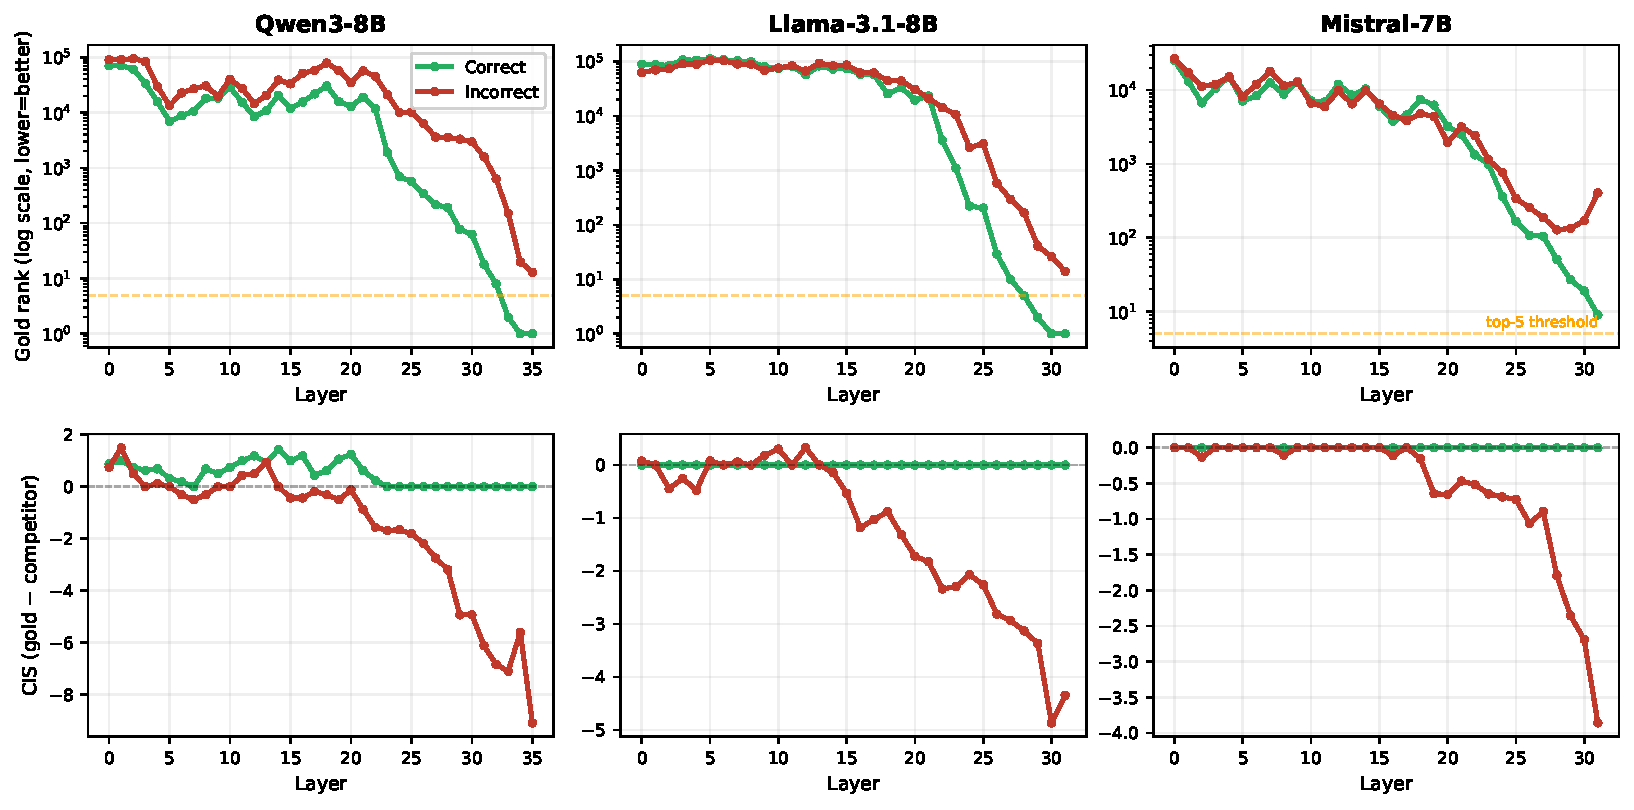
\includegraphics[width=0.95\textwidth]{figures/fig3_trajectories.pdf}
\caption{Median gold-answer rank (top, log scale) and probability margin (bottom) across layers for correct (green) and incorrect (red) predictions across model families.}
\label{fig:trajectories}
\end{figure}

\subsection{Strict Answer-Onset Preservation Failures Are a Minority}

\paragraph{Primary retrospective rate.}
Applying Eq.~8 to the first answer token of each error yields a small preservation-failure subset. On the Qwen3-8B calibrated subset, the tuned lens identifies 8.9\% (bootstrap 95\% CI [6.4\%, 11.5\%]). On the full seven-task error set (1{,}494 errors), the strict answer-onset rate is 10.0\% (95\% CI [8.4\%, 11.4\%]): multi-hop QA 14.2\% [9.5, 19.5], world knowledge 12.6\% [7.8, 18.0], long-context comprehension 12.1\% [8.0, 16.6], knowledge QA 12.0\% [8.5, 15.9], science reasoning 10.9\% [7.0, 14.8], commonsense reasoning 9.2\% [5.6, 13.3], and mathematical reasoning 0.0\%. These percentages are the paper's primary taxonomy result. They concern the answer-onset token and the endpoint-conditioned strict criterion; they are not sequence-level claims.

\begin{table}[t]
\centering
\caption{Primary strict answer-onset preservation rate on Qwen3-8B errors. The label is Eq.~8 under the stored zero-based $k=5$ cutoff. Intervals are bootstrap 95\% CIs.}
\label{tab:strict_rates}
\begin{tabular}{lrrc}
\toprule
\textbf{Task} & \textbf{Errors} & \textbf{Rate} & \textbf{95\% CI} \\
\midrule
HotpotQA & 190 & 14.2\% & [9.5, 19.5] \\
MMLU & 167 & 12.6\% & [7.8, 18.0] \\
QuALITY & 199 & 12.1\% & [8.0, 16.6] \\
TriviaQA & 283 & 12.0\% & [8.5, 15.9] \\
ARC-Challenge & 229 & 10.9\% & [7.0, 14.8] \\
CommonsenseQA & 196 & 9.2\% & [5.6, 13.3] \\
GSM8K & 230 & 0.0\% & [0.0, 0.0] \\
\midrule
\textbf{Overall} & \textbf{1{,}494} & \textbf{10.0\%} & \textbf{[8.4, 11.4]} \\
\bottomrule
\end{tabular}
\end{table}

The translator sees no gold labels, but its final-logit objective can still influence the measured absolute rate. We therefore do not describe 10.0\% as a decoder-independent ground truth. The stronger decoder-robust finding is that correct and incorrect examples remain separated under raw, tuned, and cosine readouts, while preservation failures remain a minority under the tested strict thresholds (Appendix~\ref{app:probe}).

\subsection{Counterfactual Sequence Decodability and Threshold Sensitivity}
\label{sec:taskdecay}

\paragraph{Teacher-forced results are a separate measurement.}
Appendix Table~\ref{tab:taskdecay} reports two auxiliary quantities under gold-prefix teacher forcing: ALL requires every answer token to satisfy the stored cutoff at one common intermediate layer, and Min-rule requires at least one token to enter the cutoff and later fall below rank 10. Neither column is the primary Eq.~8 preservation rate. ALL does not itself require final decay, while Min-rule changes the selected token across positions and is length-sensitive. Their disagreement is therefore a measurement-boundary result, not an alternative estimate of the same population.

The sharp QuALITY discrepancy (0.5\% under TF-ALL versus 27.6\% under Min-rule) illustrates the length problem: isolated answer tokens can become decodable without the full sequence forming coherently. For GSM8K, even the permissive Min-rule loss rate is only 5.2\%. We interpret this cautiously as a boundary of final-answer-token analysis, not proof that all mathematical errors share one mechanism.

Under the strict Eq.~8 analysis on its evaluated subset, the measured rate is 4.8\% at $k=1$, 8.5\% at $k=5$, 10.1\% at $k=10$, and 16.9\% at $k=50$. The exact percentage is threshold- and decoder-dependent, but preservation failures remain a minority across this range (Appendices~\ref{app:thresholds} and~\ref{app:probe}).

\section{Retrospective Prediction of Later Signal Decay}

\paragraph{Prediction target.}
We next ask whether trajectory shape contains information about later decay. We train a linear classifier on values observed in the first half of the network ($\ell\leq L/2$) to predict a second-half decay label. Let $t_0=\lfloor L/2\rfloor$ and define:
\begin{equation}
y^{\mathrm{decay}} = \mathbb{1}\Big[\max_{\ell \in \{t_0,\ldots,L-1\}} \mathrm{CIS}^{\mathrm{comp}}_\ell > 0 \;\;\land\;\; \mathrm{CIS}^{\mathrm{comp}}_L < 0 \Big] .
\end{equation}
The label is positive when the gold-versus-competitor margin is positive at some non-final layer in the second half and negative at the output. The feature layers and label layers do not overlap. However, $\mathrm{CIS}^{\mathrm{comp}}$ uses a competitor whose identity is selected at the final layer. The headline experiment is therefore a \emph{retrospective endpoint-conditioned prediction task}, not a strictly online forecast.

\paragraph{Trajectory history outperforms compact summaries.}
The endpoint-conditioned linear model reaches 5-fold cross-validated AUC $0.75\pm0.02$ (95\% CI [0.70, 0.80]) on Qwen3-8B. Figure~\ref{fig:prediction}a compares it with compact baselines: final-layer confidence 0.69, a direction-fixed CIS slope 0.39, midpoint rank 0.51, margin-plus-slope 0.61, and running-maximum-plus-slope 0.61. Because AUC 0.39 becomes 0.61 if the score direction is reversed, we do not interpret that value as worse-than-random evidence; it shows that the prespecified slope direction is not a reliable standalone predictor. Appendix~\ref{app:prediction} reports direction-agnostic single-feature values, including midpoint margin 0.60, margin slope 0.61, and midpoint rank 0.51. We use L2-regularized logistic regression with standardized features and stratified 5-fold cross-validation. The out-of-fold PR-AUC is 0.71 at a 46\% positive rate. A random forest reaches $0.92\pm0.01$, but we report it only as an upper bound on exploitable structure.

\paragraph{Endpoint-free and final-confidence controls.}
Final gold margin, final gold rank, and final output entropy obtain AUCs 0.67, 0.70, and 0.68; their combination reaches 0.70. More importantly, an endpoint-free variant that uses only the gold token's first-half rank, log-probability, and slopes reaches AUC 0.66. Thus, part of the 0.75 result comes from endpoint-conditioned contrast information, while a smaller but nontrivial signal remains in the gold trajectory alone.

Beyond within-task prediction, the trajectory's structure transfers in a structure-dependent way across tasks (strong between entity-style knowledge-QA datasets and from multi-hop QA into math, weak from single-step fact recall into math) and across model families (leave-one-model-out mean AUC 0.739). The gain is not explained by endpoint conditioning of the margin (an endpoint-free variant using only gold-token features still reaches AUC 0.66), nor by temporal autocorrelation (persistence and autoregressive forecasts reach only 0.56--0.62), and no single dynamic feature matches the full trajectory (strongest individual feature AUC 0.64). Full analyses, tables, and the feature-decomposition figure are in Appendix~\ref{app:prediction}.

\paragraph{Gold-free prediction within known errors.}
\label{sec:nonoracle}
The preceding predictors require the gold token. We also train a random forest using only the model's first-half five-token candidate distributions: leader churn, the fraction of prefix layers held by the midpoint leader, top-1/top-2 margins, and five-token entropy. Because pooled cross-validation over a seven-task error pool can exploit task identity and base-rate differences, we report the evaluation in three regimes. (i)~\emph{Pooled out-of-fold}: ROC-AUC 0.669 (bootstrap 95\% CI [0.630, 0.709]) and PR-AUC 0.383 at a 0.294 base rate, with a 1.35$\times$ precision lift at the top 20\%. (ii)~\emph{Within-task} 5-fold held-out evaluation, the deployment-relevant number when the trigger is calibrated on the target task: AUC 0.615 (ARC), 0.650 (GSM8K), 0.613 (MMLU), 0.526 (QuALITY), 0.488 (HotpotQA), 0.463 (TriviaQA), and 0.462 (CommonsenseQA), averaging 0.55. The gap between the pooled 0.669 and the within-task average quantifies how much of the pooled number reflects task mixture rather than per-sample signal; we therefore treat 0.55 as the honest per-sample estimate. (iii)~\emph{Task-grouped and zero-shot}: with task-grouped folds the pooled AUC falls to 0.45, and training on one task and testing on another averages 0.52, so the features do not transfer zero-shot across task types and calibration data from the target distribution is required. This is an error-subtyping experiment throughout: it assumes an upstream mechanism has already identified an answer as erroneous, and its trigger utility is demonstrated only under within-task calibration.

\begin{figure}[t]
\centering

\includegraphics[width=0.95\textwidth]{figures/fig5_prediction.pdf}
\caption{Retrospective decay prediction. (a) The endpoint-conditioned full trajectory reaches cross-validated AUC $0.75\pm0.02$; compact baselines use the labels shown on the axis. (b--c) Cross-task and cross-model transfer for the endpoint-conditioned prediction task. These panels do not evaluate an end-to-end gold-free trigger.}
\label{fig:prediction}
\end{figure}

\section{Behavioral Intervention and Component Analysis}

We next test whether the trajectory taxonomy corresponds to a behavioral difference. Our strongest control matches preservation and formation failures by final gold rank and compares restoration from their intermediate peak states. We additionally report gold-direction ablations and direction-targeted patches as oracle mechanism probes. Because these interventions are constructed from the gold token's unembedding direction, they directly favor or remove support for that token; they are not deployable repair methods or controls matched for identical direct gold-logit effects.

\paragraph{Recovery metrics.}
Two recovery metrics are used and must not be conflated. For generation-based interventions (logit bonus, representation-engineering steering, peak-state restoration, and the rank-matched experiment), recovery means the full 32-token greedy regeneration is judged correct by the standard evaluator, so a recovered example produces a semantically acceptable complete answer. For single-forward-pass patches (gold-direction patching and component-selective patching), recovery means the gold answer token attains rank 0 at the answer-onset position after one patched forward pass, matching the answer-onset taxonomy; these experiments do not regenerate the full answer.

\subsection{Direct Logit Attribution}

We use direct logit attribution \citep{elhage2021mathematical, geva2021transformer} to measure each MLP write's direct projection onto the gold-versus-competitor unembedding direction:
\begin{equation}
\Delta \mathrm{CIS}^{\mathrm{MLP}}_\ell = (w_{y^\star} - w_{y^-})^\top m_\ell(x) .
\end{equation}
Here $y^-$ is the fixed final competitor. The quantity is a local direct-effect diagnostic. Layer normalization and subsequent computation can change downstream effects, so it is not a complete causal decomposition of the final logit.

For Qwen3-8B errors, layer 35 has the largest negative direct attribution. The component interventions below show that removing margin-opposing writes from several late MLPs can increase gold-token recovery; they do not establish that layer 35 is uniquely necessary.

\paragraph{Component-level attribution: which component contributes most negatively to the gold-vs-competitor margin?}
\label{sec:components}
We also read the margin before attention, after attention, and after the MLP at each layer. Across incorrect examples, the cumulative negative contribution is $-4.71$ for MLPs and $-3.42$ for attention; the layer-35 MLP is the largest single direct contributor at $-3.42$. Correct examples show much smaller totals (attention $-0.52$, MLP $-0.51$). These diagnostics identify late MLP writes as a useful intervention site, while the adjacent-layer results below show that the effect is distributed across layers 31--35.

\subsection{Differential Repairability Under Oracle Interventions}

The simple interventions first establish expected behavior; final-rank matching provides the main control for the taxonomy. All interventions in this section use the gold answer at analysis time.

If the formation-versus-preservation distinction captures a real difference in internal state, then a targeted intervention should rescue preservation failures far more than formation failures under the same steering strength. We test this with a calibrated logit bonus: during generation, we add a fixed bonus $\beta$ to the gold token's logit at every decoding step. Because preservation failures have the gold token at final-layer rank $\le5$ in 91\% of cases (median rank 1), even a small bonus suffices to tip the gold token to the top prediction and recover the correct answer. Formation failures, by contrast, have the gold token at median rank 23, so the same small bonus cannot bridge the gap. Table~\ref{tab:steering} (Appendix~\ref{app:steering}) reports the full sweep.

At $\beta=3$, preservation failures recover at 30.0\% and formation failures at 6.4\%. This result is largely expected because the groups differ in final gold rank, and we treat it as a calibration check rather than validation of a distinct mechanism. The rank-matched experiment below addresses this confound.

We note that this experiment uses the gold token identity and is therefore an oracle proof-of-concept rather than a deployable inference-time method. Its purpose is to validate that the formation-preservation distinction corresponds to a real difference in repairability, not to propose a practical repair system. The sample counts (n=40 preservation, n=110 formation) reflect the natural class proportions among the 150 error examples evaluated on Qwen3-8B.

\paragraph{Offline representation-engineering steering.}
We construct an activation-steering pipeline whose direction is the mean hidden-state difference between correct and incorrect examples at the last four layers. The trigger uses the gold-answer trajectory and is therefore an offline oracle-assisted analysis. Selective steering achieves 9.1\% recovery per intervention versus 4.0\% for steering all errors, while ground-truth preservation and formation groups recover at 6.6\% and 1.8\%. These results are consistent with differential repairability, but the trigger and steering comparison are not final-rank matched; the paired restoration experiment below is the cleaner control.

\paragraph{Gold-free trigger within an error-only evaluation.}
The oracle-assisted trigger above gives a 127\% efficiency gain. With the gold-free predictor of Section~\ref{sec:nonoracle}, calibrated per task on labeled errors and evaluated on a task-balanced error set, selective steering recovers 9.5\% per intervention versus 5.7\% for indiscriminate steering at 20\% coverage. Trigger precision is 64\% against a 33\% base rate. This experiment still conditions on an error-only pool and therefore demonstrates subtyping utility, not a complete deployment pipeline.

\paragraph{Peak-state restoration decouples repairability from final rank.}
We first intervene on the intermediate state rather than the output. For each error, we identify the layer $L^\star$ where the gold rank peaks, capture the last-token residual at $L^\star$, and blend subsequent residuals toward it: $h_\ell'=(1-\alpha)h_\ell+\alpha h_{L^\star}$. At $\alpha=0.8$, preservation failures recover at 8.3\% and formation failures at 3.3\%; at $\alpha=0.5$, the rates are 5.0\% and 0.0\%. This is consistent with the distinction, but final-rank differences remain, motivating a matched analysis.

\paragraph{Rank-matched intervention.}
We match each preservation failure to a formation failure with peak gold rank $>20$ and final gold rank within $\pm3$, then apply the same peak-state restoration. The groups have median final ranks 8 and 11 but median peak ranks 3 and 31. At $\alpha=1$, recovery is 12.3\% versus 1.8\% (57 matched pairs; paired bootstrap 95\% CI for the difference [1.8\%, 19.3\%]; McNemar exact $p=0.070$). The rate ratio grows with restoration strength, and an output-logit bonus on the same pairs does not separate the groups. Because the exact paired test does not cross 0.05 and the sample is modest, we treat this as directional matched evidence rather than a statistically decisive result.

\paragraph{Gold-direction activation patching.}
\label{sec:causal-patch}
The layer-35 attribution is correlational, so we restore the gold-direction component that decayed from the peak state:
$h_\ell'=h_\ell+\beta\,\mathrm{clamp}_{\ge0}((h_{L^\star}-h_\ell)^\top\hat w_{y^\star})\hat w_{y^\star}$.
Among examples not already top-1, the patch recovers 7.3\% of preservation failures and 0.7\% of formation failures ($p=0.005$), versus 0/109 for an orthogonal random-direction control ($p=0.003$). The control shows direction specificity relative to a norm-like perturbation, but it is not matched for the same direct first-order increase in the gold logit. We therefore conclude narrowly that restoring support along the gold unembedding direction can recover some preservation failures.

\paragraph{Component-selective, direction-targeted patching.}
We next delete the margin-opposing part of a single component write,
$m'=m-\gamma\,\mathrm{clamp}_{\le0}(m^\top\hat d)\hat d$,
where $\hat d$ is the unit gold-versus-competitor direction. On preservation failures, the layer-35 MLP patch recovers 11.0\%, 20.2\%, and 31.2\% at $\gamma=1,2,4$, while an orthogonal random direction recovers 0/109. Adjacent MLPs recover similarly (layer 34: 12.8--33.0\%; layer 33: 11.9--25.7\%; layer 31: 4.6--22.0\%), and full zero-ablation performs worse. These results show that late MLP writes contain margin-opposing components whose removal can increase gold-token recovery, and that this opportunity is distributed across layers 31--35. Because the target direction is explicitly constructed from the gold and competitor unembeddings, the experiment does not prove that the network contains a uniquely identifiable semantic ``correct-answer variable'' or that the intervention can be selected without oracle information.

\section{InfoDyn-Bench}

We construct \texttt{InfoDyn-Bench}, a benchmark of layered information trajectories for LLM error analysis. Unlike resources that store only final outputs or static activations, it records the full per-layer gold-answer trajectory alongside explicitly versioned derived labels. Table~\ref{tab:benchmark} summarizes its intended contents. It covers six models across three families and seven tasks, with raw and tuned-lens trajectories, derived dynamics metrics, taxonomy labels, and prediction splits.

Researchers can use the benchmark to compare decoder-dependent taxonomy labels, reproduce retrospective prediction analyses, and select candidates for intervention studies. Because the manuscript distinguishes answer-onset Eq.~8 labels from teacher-forced sequence diagnostics, the release must store the defining metric, cutoff, answer position, and decoder with every label rather than exposing a single ambiguous ``preservation'' field.

% AUTHOR ACTION REQUIRED BEFORE SUBMISSION:
% Insert an anonymous artifact URL and report the exact released sample count,
% licenses, checksums/version, and which of the six-model x seven-task cells
% contain full raw+tuned trajectories rather than summary-only results.

\section{Discussion and Limitations}

\paragraph{What does ``the model knows'' mean?}
Competitive decodability is an operational sign of output readiness, not a complete definition of knowledge. In particular, satisfying the $k=5$ rank cutoff does not imply semantic knowledge, and failing it does not imply that relevant information is absent from every position or nonlinear feature of the network.

\paragraph{Different failures call for different interventions.}
The taxonomy suggests hypotheses rather than prescriptions. Errors without an output-competitive gold token might benefit from retrieval, reasoning correction, or editing \citep{meng2022rome}; errors with a transient competitive token are plausible candidates for retention-style interventions \citep{turner2023activation, zou2023representation}. The present evidence is oracle-assisted and does not establish that either treatment is optimal at deployment time.

\paragraph{Why do trajectories predict?}
We conjecture that the slope reflects signal stability, the early peak reflects formation speed, and the fluctuation reflects the competitive state. History therefore separates a transient fluctuation from a stable formation better than a single snapshot.

\paragraph{Limitations.}
Our primary taxonomy is retrospective and answer-onset based. It depends on an endpoint-selected competitor and a decoder-specific threshold, and the tuned lens is trained toward final logits. The teacher-forced sequence analysis is counterfactual because later answer tokens are conditioned on gold prefixes that were not generated in the original error. The gold-free predictor is evaluated within known errors, not jointly on error detection and subtype selection. The interventions use gold or gold-versus-competitor directions and are not matched for identical direct effects on the gold logit; their strongest conclusions are therefore direction-specific and oracle-assisted. Correctness is determined by normalized substring/numeric matching rather than exhaustive human adjudication. Finally, our models span 4B--14B parameters and do not include larger or reasoning-specialized systems.

\section{Conclusion}

We showed that pairwise crossing against one wrong token cannot establish that a gold answer was ever vocabulary-competitive. Under a stricter answer-onset criterion, a small, task-dependent subset of errors exhibits a competitive intermediate gold token that is not preserved to the output. Retrospective trajectory features predict this later decay, although the strongest predictor is endpoint-conditioned, and final-rank-matched restoration gives directional evidence that the identified subset is more repairable. These conclusions concern decoded output-space dynamics rather than a complete account of knowledge or reasoning. We release \texttt{InfoDyn-Bench} to support more controlled studies of layer-wise error diagnosis.

\appendix

\section{Metric Usage}
\label{app:metric}

\begin{table}[h]
\centering
\caption{Measurement object used by each analysis. The strict taxonomy and full prediction model are endpoint-conditioned through $y^-$.}
\label{tab:metric}
\begin{tabular}{ll}
\toprule
\textbf{Analysis} & \textbf{Object} \\
\midrule
Endpoint selection bias & $\mathrm{CIS}^{\mathrm{gen}}$ \\
Correct versus incorrect comparison & $\mathrm{CIS}^{\mathrm{comp}}$ \\
Competitive-decay classification & $\mathrm{CIS}^{\mathrm{comp}}$ \\
Full retrospective prediction & $\mathrm{CIS}^{\mathrm{comp}}$ \\
Endpoint-free prediction & Gold rank and log-probability \\
Direct logit attribution & $\mathrm{CIS}^{\mathrm{comp}}$ \\
\bottomrule
\end{tabular}
\end{table}

\section{Probe Robustness, Label Leakage, and Lens Agreement}
\label{app:probe}

\paragraph{Probe robustness across independent decoders.}
To confirm that this intermediate rank separation is a genuine property of the internal representations rather than an artifact of the raw logit lens, we recomputed peak intermediate ranks under three independent decoding methods: the raw logit lens, the tuned lens, and a parameter-free cosine similarity between intermediate hidden states $h_\ell$ and unembedding vectors $w_{y^\star}$. Across all three decoders, correct and incorrect predictions remain separated by over an order of magnitude in rank (medians 0 vs. 32 for raw lens, 0 vs. 12 for tuned lens, 1 vs. 43 for training-free cosine similarity; Mann-Whitney $p < 10^{-20}$ in all cases). Because cosine similarity uses no learned parameters or final layer normalization, the separation is robust across multiple readout methods and is not an artifact of any single decoder.

\paragraph{No answer-label leakage, but final-output alignment.}
The tuned-lens translators are trained on 200 held-out unlabelled prompts (one affine map per layer, trained independently with Adam, learning rate $10^{-3}$, 500 epochs) to predict the model's final-layer logits, and never observe gold answers or correctness labels. This rules out answer-label leakage, but not decoder bias: the target is the final output distribution, including the final wrong distribution on errors. We therefore treat tuned-lens rates as decoder-conditional and retain raw and cosine readouts as robustness checks. Because the per-example taxonomy labels under the three decoders were not stored for all model-task cells, we report decoder robustness at the level of the correct-versus-incorrect separation (above) rather than as sample-level label agreement; absolute preservation rates remain conditional on the decoder.

\paragraph{Raw versus tuned lens comparison.}
The raw lens produces peak margins about $2.0\times$ larger than the tuned lens, while both preserve the aggregate ordering between correct and incorrect examples. This agreement supports the qualitative separation but does not establish sample-level taxonomy invariance; absolute rates remain conditional on the chosen decoder.

\section{Threshold Sensitivity and Measurement Boundaries}
\label{app:thresholds}

\paragraph{Robustness across competitiveness thresholds.}
We re-evaluated the strict competitive-decay rate across stored zero-based cutoffs $k \in \{1,5,10,50\}$ on the Qwen3-8B analysis subset while holding $\mathrm{CIS}^{\mathrm{comp}}_\ell>0$ fixed. The rate is 4.8\%, 8.5\%, 10.1\%, and 16.9\%, respectively. The exact prevalence is cutoff-dependent, but the qualitative conclusion that this is a minority regime is stable over the tested range. The full seven-task 10.0\% figure is computed on a different, larger error set and should not be numerically equated with the subset's 8.5\%.

\paragraph{Measurement boundaries on multi-step reasoning.}
The 5.2\% GSM8K value in Table~\ref{tab:taskdecay} is the permissive Min-rule loss diagnostic, not the strict Eq.~8 preservation rate, which is 0.0\% on the reported seven-task analysis. Computing the best rank across all gold-answer tokens also gives 5.2\%, partly because many GSM8K answers are single-token numbers. This does not establish that mathematical errors never contain relevant intermediate reasoning states; it shows that final-answer-token tracking rarely exposes the tested decay pattern. Studying intermediate calculations is outside the scope of the present taxonomy.

\begin{table}[h]
\centering
\caption{Counterfactual teacher-forced sequence diagnostics on Qwen3-8B errors. TF-ALL measures simultaneous intermediate formation under a gold prefix; Min-rule loss measures whether any answer token satisfies $r\leq5$ and later falls below rank 10. Neither is the primary Eq.~8 preservation label. The overall Min-rule value is the error-count-weighted aggregate of the displayed task rates.}
\label{tab:taskdecay}
\begin{tabular}{lrrr}
\toprule
\textbf{Task} & \textbf{Errors} & \textbf{TF-ALL} & \textbf{Min-rule loss} \\
\midrule
HotpotQA & 190 & 24.2\% & 26.3\% \\
TriviaQA & 283 & 23.0\% & 27.9\% \\
MMLU & 167 & 16.8\% & 23.4\% \\
ARC-Challenge & 229 & 12.2\% & 23.6\% \\
CommonsenseQA & 196 & 9.7\% & 12.2\% \\
GSM8K & 230 & 4.3\% & 5.2\% \\
QuALITY & 199 & 0.5\% & 27.6\% \\
\midrule
\textbf{Overall} & \textbf{1{,}494} & \textbf{13.2\%} & \textbf{20.9\%} \\
\bottomrule
\end{tabular}
\end{table}

\section{Prediction: Additional Analyses}
\label{app:prediction}

\paragraph{Endpoint conditioning and its scope.}
We note that the competitive margin $\mathrm{CIS}^{\mathrm{comp}}_\ell$ is defined with respect to the final-layer competitor $y^-$, so the first-half features are not purely endpoint-free: the identity of the eventual competitor is determined at the final layer. To quantify the contribution of this endpoint conditioning, we re-trained the predictor using only features that do not reference $y^-$ (the gold log-probability, gold rank, and their slopes, which depend only on the gold token itself). This endpoint-free predictor still achieves AUC 0.66, which remains above all single-layer baselines and temporal-extrapolation baselines (persistence 0.60, AR 0.62), showing that the gold-answer trajectory alone carries predictive signal about future decay. The full trajectory's higher AUC (0.75) reflects additional information from the gold-vs-competitor contrast, which is a legitimate trajectory quantity but does depend on which token ultimately wins. All baselines in our comparison use the same CIS definition, so the relative ordering (full trajectory $>$ AR $>$ persistence) is not affected by this conditioning.

\paragraph{Structure-dependent cross-task generalization.}
As illustrated in Figure~\ref{fig:prediction}b, decay prediction transfers across tasks in a structure-dependent manner. Transfer is strong between entity-style knowledge QA datasets (TriviaQA $\to$ HotpotQA, AUC 0.74) and from multi-hop QA to multi-step math reasoning (HotpotQA $\to$ GSM8K, AUC 0.77). Conversely, transfer from single-step fact recall to multi-step reasoning is weaker (TriviaQA $\to$ GSM8K, AUC 0.38), consistent with our finding that GSM8K final-answer tokens do not form intermediate competitive signals (Section~\ref{sec:taskdecay}). Using a nonlinear classifier (random forest), the strongest cross-task direction (TriviaQA $\to$ HotpotQA) reaches 0.86, confirming that the transferable signal is not saturated by the linear model.

\paragraph{Robust cross-model transfer across architectures.}
To test whether trajectory dynamics reflect shared Transformer properties, we evaluated cross-model transfer across three distinct model families, reporting the results in Table~\ref{tab:crossmodel} and Figure~\ref{fig:prediction}c. All model pairs exceed chance (0.5), with Qwen3-8B $\to$ Llama-3.1-8B reaching AUC 0.728 and Llama-3.1-8B $\to$ Mistral-7B reaching 0.779; the weakest cross-family direction (Mistral-7B $\to$ Llama-3.1-8B) is 0.599, still above chance. Leave-one-model-out transfer averages AUC 0.739. By aligning layers by relative depth and applying normalization strictly on training models, these results show that the trajectory pattern transfers across the evaluated Transformer families rather than being a single-model fitting artifact.

\begin{table}[h]
\centering
\caption{Cross-model decay-prediction AUC across model families. Rows indicate training models, and columns indicate test models.}
\label{tab:crossmodel}
\begin{tabular}{lccc}
\toprule
\textbf{Train $\backslash$ Test} & Qwen3-8B & Llama-3.1-8B & Mistral-7B \\
\midrule
Qwen3-8B & \cdot & \textbf{0.728} & 0.748 \\
Llama-3.1-8B & 0.695 & \cdot & 0.779 \\
Mistral-7B & 0.639 & 0.599 & \cdot \\
\midrule
Leave-one-out & 0.703 & 0.750 & 0.763 \\
\bottomrule
\end{tabular}
\end{table}

\paragraph{Trajectory decomposition: Dynamic shape drives prediction.}
To isolate which properties contribute to prediction, we evaluate individual features (Figure~\ref{fig:trajdecomp}). No single feature matches the full trajectory. Margin sign oscillations and peak first-half margin reach AUC 0.64, first-half variance 0.63, margin slope 0.61, midpoint margin 0.60, and midpoint rank 0.51. Combining peak, slope, and variance reaches 0.70, while the full feature set reaches 0.75. This pattern is consistent with useful information in joint trajectory shape, although all margin-based results remain endpoint-conditioned.

\begin{figure}[h]
\centering
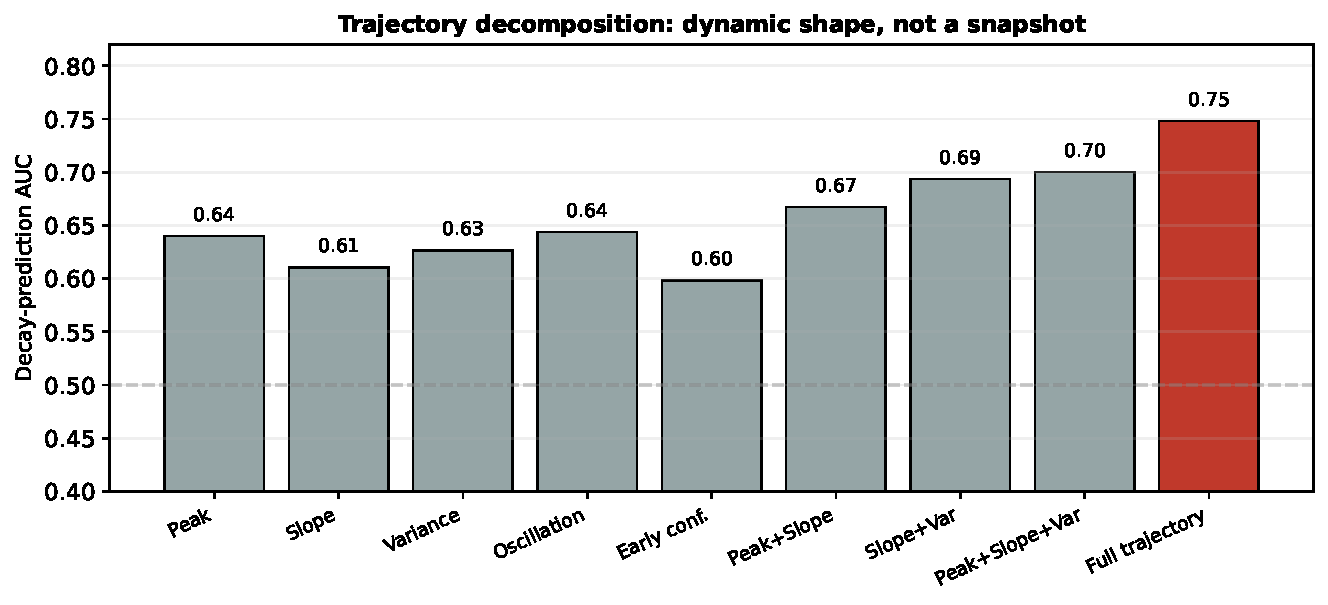
\includegraphics[width=0.95\textwidth]{figures/fig_traj_decomp.pdf}
\caption{Trajectory feature decomposition. Individual dynamic features (peak, slope, variance, transitions) outperform static snapshots, while their combination drives full predictive power.}
\label{fig:trajdecomp}
\end{figure}

\paragraph{The gain is not mere temporal autocorrelation.}
Because the decay label describes the second half of the very trajectory that the first half summarizes, one might suspect the AUC is trivially explained by temporal continuity. To test this, we compared against standard time-series forecasts computed from the first half alone: the last observed value (persistence, AUC 0.60), the first-half linear slope (0.58), linear extrapolation to the final layer (0.58), a first-order autoregressive forecast (0.62), and the first-half mean as a smoothing prior (0.56). All of these lie well below the full-trajectory linear classifier ($0.75 \pm 0.02$). If the predictive signal were just autocorrelation, an autoregressive or extrapolation baseline should approach the full-trajectory model; it does not. The additional predictive power therefore comes from the joint shape of the trajectory, not from simple temporal continuity.

\section{Gold-Direction Ablation and Norm-Matched Controls}
\label{app:ablation}

\paragraph{Behavioral necessity of the gold direction.}
We asked whether the correct-answer signal is behaviorally necessary, meaning whether removing it changes the output. We removed the component of the hidden state that lies along the gold token's unembedding direction $w_{y^\star}$ (defined in Section~\ref{sec:def}) in the last three layers:
\begin{equation}
h'_\ell = h_\ell - \operatorname{proj}_{w_{y^\star}}(h_\ell) .
\end{equation}
Here $\operatorname{proj}_{w_{y^\star}}(h_\ell)$ is the projection of $h_\ell$ onto $w_{y^\star}$, so the operation deletes the part of the representation that pushes toward the gold token. We applied this to examples that were originally correct and measured how many flipped to wrong.

The ablation flips correct examples to wrong at high rates across all models, as Table~\ref{tab:ablation} shows.

\begin{table}[h]
\centering
\caption{Behavioral necessity across model families and scales. Ablating the gold direction flips correct examples to wrong at high rates, while a random-token control flips almost none. Parentheses give Wilson 95\% intervals for the gold flip rate.}
\label{tab:ablation}
\begin{tabular}{lcccc}
\toprule
\textbf{Model} & \textbf{Baseline correct} & \textbf{Gold flip} & \textbf{Random token flip} \\
\midrule
Qwen3-14B & 30/30 & 23/30 (77\%, CI [59, 88]) & 0/30 (0\%) \\
Qwen3-8B & 50/50 & 38/50 (76\%, CI [63, 86]) & 0/50 (0\%) \\
Qwen3-4B & 27/27 & 18/27 (67\%, CI [48, 81]) & 0/27 (0\%) \\
Qwen2.5-7B & 30/30 & 26/30 (87\%, CI [70, 95]) & 1/30 (3\%) \\
Llama-3.1-8B & 30/30 & 22/30 (73\%, CI [56, 86]) & 0/30 (0\%) \\
Mistral-7B & 30/30 & 12/30 (40\%, CI [25, 58]) & 0/30 (0\%) \\
\bottomrule
\end{tabular}
\end{table}

The gold flip rates are 77\%, 76\%, 67\%, 87\%, 73\%, and 40\% for Qwen3-14B, Qwen3-8B, Qwen3-4B, Qwen2.5-7B, Llama, and Mistral. The random-token control flips 0\% in almost every model (one example in Qwen2.5-7B). The effect is consistent across model families and across scales from 4B to 14B. The difference between the strongest model (Qwen2.5-7B, 87\%) and the weakest (Mistral-7B, 40\%) is statistically distinguishable: their 95\% intervals, [70, 95] and [25, 58], do not overlap, so the variation across architectures is not merely sampling noise.

\paragraph{Norm-matched controls.}
To check that the effect is not just any direction change, we ablated other directions. A key concern is that the gold unembedding direction is the main source of the gold log-probability, so removing it lowers that log-probability more than removing any other direction would. To make the comparison fair, we matched the \emph{perturbation magnitude}: for each control direction, we set the per-layer removal strength so that the hidden-state change $\lVert \Delta h \rVert$ equals that of the gold ablation. This way all interventions change the representation by the same amount and differ only in which direction they remove.

Under this norm-matched protocol, the gold direction flips more examples than the controls across Qwen scales. On Qwen3-8B, gold flips 83.3\% of correct examples, while the second-best candidate flips 38.9\%, a random token 5.6\%, and a random Gaussian direction 11.1\%. On Qwen3-4B, the corresponding rates are 70.0\%, 35.0\%, 15.0\%, and 5.0\%. On Qwen3-14B, they are 75.0\%, 55.0\%, 5.0\%, and 0.0\%. Matching $\lVert\Delta h\rVert$ rules out a generic perturbation-size explanation, but it does not match the directions' direct first-order effects on the gold logit. We therefore interpret the experiment as a direction-specific sanity check, not a complete causal control.

\section{Calibrated Logit-Bonus Steering Sweep}
\label{app:steering}

\begin{table}[h]
\centering
\caption{Oracle logit-bonus calibration. A fixed bonus $\beta$ is added to the gold token. The groups are not matched by final gold rank, so the ratio is a sanity check rather than evidence of a distinct mechanism.}
\label{tab:steering}
\begin{tabular}{lccc}
\toprule
\textbf{Bonus $\beta$} & \textbf{Preservation (n=40)} & \textbf{Formation (n=110)} & \textbf{Ratio} \\
\midrule
1.0 & 2.5\% & 0.9\% & 2.8$\times$ \\
2.0 & 12.5\% & 2.7\% & 4.6$\times$ \\
3.0 & 30.0\% & 6.4\% & 4.7$\times$ \\
5.0 & 32.5\% & 11.8\% & 2.8$\times$ \\
\bottomrule
\end{tabular}
\end{table}

\section{InfoDyn-Bench Contents}
\label{app:bench}

\begin{table}[h]
\centering
\caption{Contents of \texttt{InfoDyn-Bench}. Each example stores the per-layer trajectory and derived labels; the benchmark is organized so that each downstream use case maps to a stored field.}
\label{tab:benchmark}
\small
\begin{tabular}{lp{8.6cm}}
\toprule
\textbf{Component} & \textbf{Description} \\
\midrule
\textbf{Input} & Question, gold answer, aliases, generated answer, correctness label. \\
\textbf{Trajectory} & Per-layer gold-answer log-probability, full-vocabulary rank, and competitor-relative margin under raw and tuned lenses. \\
\textbf{Derived metrics} & Signal-emergence layer (SEL), peak rank, peak margin, dwell time, peak-to-final decay, sign-change flag, and $k=5$ cutoff entry. \\
\textbf{Failure label} & Operational labels with the defining metric and decoder recorded; the primary paper label is answer-onset Eq.~8. \\
\textbf{Prediction split} & $t_0$ prefix features, the $y^{\mathrm{decay}}$ label (does the signal decay in the second half?), and final correctness. \\
\textbf{Coverage} & 6 models (Qwen3-4B/8B/14B, Qwen2.5-7B, Llama-3.1-8B, Mistral-7B) $\times$ 7 tasks (TriviaQA, HotpotQA, GSM8K, CommonsenseQA, ARC-Challenge, QuALITY, MMLU). \\
\bottomrule
\end{tabular}
\end{table}


\bibliography{iclr2027_conference}
\bibliographystyle{iclr2027_conference}

\end{document}
